% This is the template for submission of abstracts to NetSci 2024 in Québec, Canada.
% It is modified from NetSci2017, which was inspired by that of NetSci2016 and that of STATPHSY25.
% The editor of the booklet reserves the right to modify your submission.

% To process this file run LaTeX2e

% ******** DO NOT EDIT ****************
\documentclass[10pt]{article}
% \usepackage{mathptmx}
\usepackage[letterpaper,margin=20mm]{geometry}
\usepackage{graphicx}
\usepackage{lmodern}
\renewcommand{\familydefault}{\sfdefault}
\pagestyle{empty}
\setlength{\parskip}{0.25\baselineskip}
\renewcommand{\title}[1]{{\noindent\large\bfseries#1\medskip\\}}
\renewcommand{\author}[2]{{\noindent #1 \medskip\\ \noindent \small #2 \medskip\\}}
% *************************************

\begin{document}

% ********** USER DEFINED *************


% Enter title here
\title{Welcome to NetSci 2024}
\author{
    % Enter author(s) here
    A. Allard,\textsuperscript{1}
    L. H\'ebert-Dufresne,\textsuperscript{2}
    J. Lovato,\textsuperscript{2}
    A. Patania,\textsuperscript{2}
    G. St-Onge,\textsuperscript{3}
    and
    J.-G. Young\textsuperscript{2}
}
{
    % Enter affiliation(s) here
    1. Universit\'e Laval, Qu\'ebec, Canada\\
    2. University of Vermont, Burlington, VT, USA\\
    3. Northeastern University, Boston, MA, USA
}



% Enter abstract here. Please keep everything within one page.
It is an honor and pleasure to invite the network science community to NetSci 2024 in Québec City from June 16th to 21st 2024.

Québec City has a rich history, mix of culture, and sense of community that reflects our field in many ways. Founded in 1608, the city is famous for its European character and magnificent landscapes, which make it a highly valued and internationally recognized tourist destination. Québec City also proudly appears on UNESCO’s World Heritage List. The Québec City Convention Centre is located in the heart of the City by the historic district of Old Québec. Many scientific and artistic projects were born in the surrounding world‐class hotels, quaint restaurants, storied breweries, coffee shops, and green parks.

As always, NetSci 2024 will be the flagship conference of the Network Science Society and will provide an unmatched venue for sharing and discussing discoveries, ideas, and emerging problems in network science. The conference program will be broad, covering the many ways in which networks shape our world, including social networks, epidemics, ecology, neuroscience, and artificial intelligence.

The local, program and advisory committees are working to prepare an exciting and outstanding conference. Québec has a special place in the heart of many members of our community, and we can’t wait to share this unique city with new and old friends.

We look forward to welcoming you for NetSci 2024 in the beautiful city of Québec!



\bigskip
{\small
    \noindent[1] You may add a reference.\\
    \noindent[2] You may add a reference.\\
    \noindent[3] You may add a reference.
}



\begin{figure}[!h]
    \centering
    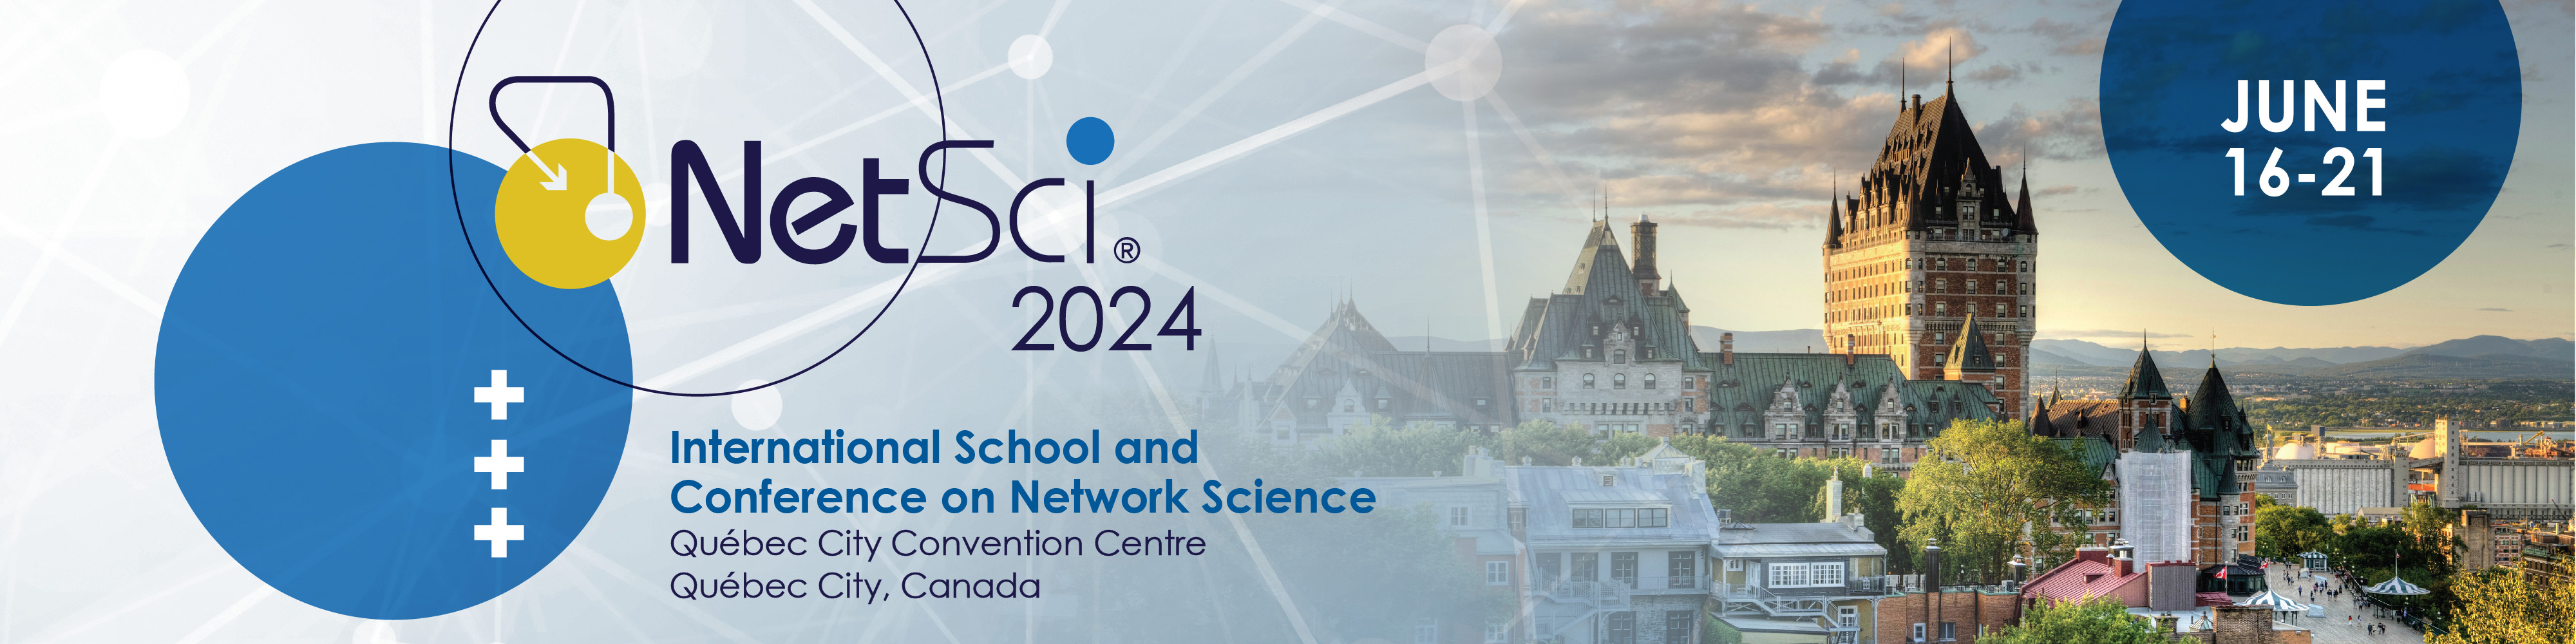
\includegraphics[width=0.8\textwidth]{NETSCI-2024_web_4000X1000.jpg}
    \caption{\textbf{Abstract must include a figure.} NetSci 2024's web banner.}
\end{figure}



% *************************************
\end{document}